%% ----------------------------------------------------------------------
%% START OF FILE
%% ----------------------------------------------------------------------

\chapter{绪论}
\label{cha:introduction}

\section{研究背景}
\label{sec:background}

日新月异的计算机技术发展,带来了数据存储设备容量和CPU处理能力的大幅度提升。然而,磁盘系统的数据带宽以及I/O吞吐率的增长速度并未跟上CPU的步伐。与之而来的是CPU和传统磁盘系统的间愈发加大的速度差距(图\ref{fig:cpu-disk-diff})。

\begin{figure}[H]
\centering
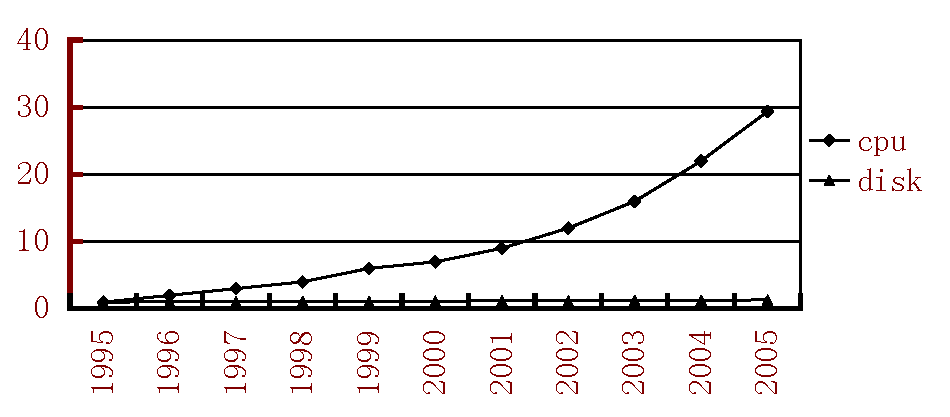
\includegraphics[width=0.7\linewidth]{./graph/cpu-disk-gap}
\caption{CPU与磁盘速度差异}
\label{fig:cpu-disk-diff}
\end{figure}

云端计算是继计算机系统从二十世纪80年代的大型计算机到“客户端-服务器”模式的又一次转变。与之而来的是对存储设备厂商对大数据(Big Data)越来越多的关注。大数据之所以会出现,是因为我们生活在一个拥有海量数据的信息社会中,21世纪人们与数据或信息交互比历史上的任何时期都要活跃。46亿全球移动电话用户中,有20亿人访问互联网,人们在畅游互联网的过程中,会自觉或不自觉的产生日志、访问历史和评论等信息,互联网上流动的交通量已经达到每年667艾字节。除了互联网,数据已经渗透到每一个行业和业务职能领域,并逐渐成为重要的生产因素。2011年5月全球知名咨询公司麦肯锡全球研究院发布了一份题为《大数据:创新、竞争和生产力的下一个新领域》的报告,报告指出了人们对于大数据的运用预示着新一波生产率增长和消费者盈余浪潮的到来。

大数据对存储系统的容量、速度及可靠性提出了非常高的要求,一些高性能的存储设备由此产生。固态硬盘(SSD)作为其中的佼佼者被引入传统的以机械硬盘(HDD)为主的存储系统。固态硬盘的读写性能远远高于传统的机械硬盘(表\ref{tab:ssd-speed-compare}),将固态硬盘引入存储系统中,将大大提高系统的性能。

\begin{table}[H]
\centering
\caption{HDD、DRAM和SSD的读写速度比较}
\begin{tabular}{|c|c|c|c|}
\hline  & Hard Disk & DRAM & SSD \\
\hline Read Access & 8.3ms & 60ns & 85ns \\
\hline Write Access & 9.1ms & 60ns & 4-10ms \\
\hline
\end{tabular}
\label{tab:ssd-speed-compare}
\end{table}

然而固态硬盘的价格仍然昂贵,虽然过去几年固态硬盘的价格一直快速下降,但下跌趋势正日益放缓,一系列问题导致固态硬盘和机械硬盘之间的价格差距不可能会很快消失。因此,固态硬盘不会在短时间内取代机械硬盘成为企业的主储存设备。固态硬盘的价格从2005年和2006年的3美元/GB跌至了2012年的0.67美元/GB,但与HDD的0.09美元/GB相比仍然相去甚远。根据固态硬盘历史价格的下降速度计算,到2020年它的价格约为0.15美元/GB,而届时机械硬盘的价格将会降至0.03美元/GB,对存储厂商来说机械硬盘仍然存在难以抗拒的价格优势。

综上,鉴于固态硬盘的价格较高且存储密度与机械硬盘差距较大,目前来讲,完全使用固态硬盘作为存储设备条件还不够成熟。虽然已有一些云计算存储中心部署了全固态硬盘的存储阵列,但是过高的成本令大多数使用者望而却步。为此,本文设计了一种既能保证成本在可接受的范围内,又能充分利用固态硬盘高IO性能的解决方案。

\section{相关研究工作}
\label{sec:related_works}

针对固态硬盘价格高、容量小、功耗低等特点,很多公司和研究者针对固态硬盘的使用场景,提出了基于固态硬盘的混合或分级存储解决方案。这些方案与全固态硬盘解决方案相比价格更能被接受。同时,相比于传统的使用DRAM作为缓冲区,基于NAND或NOR的固态硬盘有着功耗低(表\ref{tab:ssd-power-compare})、存储密度高以及可扩展性强的优势。

\begin{table}[H]
\centering
\caption{DRAM、Flash功耗比较}
\begin{tabular}{|c|c|c|c|}
\hline
\diagbox{介质}{功耗} & Density-Gb/cm2 & Active Power* & Idel Power* \\
\hline DDR2 DRAM & 0.7 & 878mW & 80mW \\
\hline NOR & 0.75 & 86mW & 16μW \\
\hline NAND & 1.42 & 28mW & 6μW \\
\hline
\end{tabular}
\\ * Power consumed for 1Gbit of memory
\label{tab:ssd-power-compare}
\end{table}

全球第六大企业软件公司EMC在2012年推出了VFCache解决方案。VFCache通过拦截不超过64KB大小的I/O请求(通常为随机操作)并将其缓存到PCIe闪存卡,从而达到加速访问的效果。由于不缓存应用程序的写操作,而是直接通过FCHBA卡写入后端SAN存储并等待其反馈成功信息,因此VFCache即便出现硬件故障也不会导致数据丢失。通过将固态硬盘引进存储阵列,EMC成为第一家涉足服务器PCIe闪存市场的主流厂商。

华为的云计算存储部门提出了解决方案SmartCache。SmartCache是一种将固态硬盘作为缓存资源的分层存储技术,是华为的一个动态数据缓存解决方案。SmartCache通过充当内存的扩展的方式,显著降低延迟并加快随机IO敏感性应用程序的执行速度,而无需以物理方式将数据移动到固态硬盘上。使用一个或多个固态硬盘作为磁盘阵列的缓存,称为SmartCache缓存池。统计HDD访问的热点数据,每隔一段时间移动到SSD的缓存池中。当热数据被访问时,就可以直接从缓存池中读取。该方案主要适用于IO请求中大部分为读,存在热点数据区域,且主要是位置随机的小请求的场景。

LSI作为一家知名的RAID适配器公司,推出了型号为LSI MegaRAID的SATA+SAS RAID控制卡。该RAID卡采用固态硬盘作为磁盘阵列的Cache存储热数据,从而有效提高读写性能,降低I/O时延,缩短RAID的访问和重建时间。结合LSI MegaRAID CacheCade Pro2.0软件,可以动态地将热数据从HDD阵列到SSD高速缓存中,操作完全透明,无需进行手动配置。

FC/SAS企业级闪存驱动器制造商STEC开源了Linux系统的EnhanceIO SSD缓存软件,能够加速任意类型的块存储设备——DAS/RAID/iSCSI/FC SAN。此外,EnhanceIO可以支持任意品牌型号的固态硬盘(包括SAS、SATA、PCIe和 Fibre Channel)作为缓存,同时针对STEC的产品有优化。缓存策略方面,EnhanceIO具备Read Cache(读缓存)、Write Back Cache(写回)和Write-through Cache(写通)三种模式,并能够在异常断电时阻止用户数据的丢失。

另一家SSD生产厂商,STEC的竞争对手Fusion-io也提出了自己的固态硬盘混合存储解决方案Fusion-io ioControl hybrid storage solution。与STEC不同的是,该解决方案针对云计算,能够很好的与虚拟机平台VMware Workstation以及Microsoft SQL Server clusters整合在一起,减少虚拟机和数据库查询的响应延迟。

\section{全文组织结构}
\label{sec:organization}

本文提出并实现了一种固态硬盘用作传统机械硬盘缓存的解决方案,在保证系统正确性和稳定性的前提下,考虑存储系统性能的提升。

全文组织结构如下。

第一章:绪论。论述当前云计算和大数据处理背景下对于存储系统性能的需求。对论文研究的意义以及国内外的相关研究工作加以简单描述。

第二章:相关技术简介。介绍与论文关系紧密的相关软硬件技术,包括SSD原理和特性、缓存系统的发展和评估、混合存储系统的原理和分类。

第三章:关键技术。介绍实现论文提出解决方案的实现中所涉及的关键技术,包括磁盘IO的捕获方式、缓存系统使用的页面替换算法、映射策略和索引结构以及缓存系统的两种回写策略。

第四章:缓存系统的实现细节。描述论文抽象出的Cache替换算法公共接口,并对每个接口的具体实现细节加以介绍。

第五章:实验和结果分析。从稳定性和性能两个角度对实现的系统进行测试,分析测试结果。于商业系统软件进行性能比较。

第六章:总结与展望。总结论文的研究成果和解决方案的贡献,展望进一步提升系统性能的改进方法。

%% ----------------------------------------------------------------------
%%% END OF FILE
%% ----------------------------------------------------------------------